\documentclass[12pt]{report}
\usepackage[spanish]{babel}
\usepackage[utf8]{inputenc}
\usepackage{amsmath}
\usepackage{amssymb}
\usepackage{amsthm}
\usepackage{graphics}
\usepackage{subfigure}
\usepackage{lipsum}
\usepackage{array}
\usepackage{multicol}
\usepackage{enumerate}
\usepackage[framemethod=TikZ]{mdframed}
\usepackage[a4paper, margin = 1.5cm]{geometry}
\usepackage{tikz}
\usepackage{pgffor}
\usepackage{ifthen}
\usepackage{enumitem}
\usepackage{hyperref}

%Gestión de Hipervínculos

\hypersetup{
    colorlinks=true,
    linkcolor=black,
    filecolor=magenta,      
    urlcolor=cyan
}

\usetikzlibrary{shapes.multipart}

\newcounter{it}
\newcommand*\watermarktext[1]{\begin{tabular}{c}
    \setcounter{it}{1}%
    \whiledo{\theit<100}{%
    \foreach \col in {0,...,15}{#1\ \ } \\ \\ \\
    \stepcounter{it}%
    }
    \end{tabular}
    }

\AddToHook{shipout/foreground}{
    \begin{tikzpicture}[remember picture,overlay, every text node part/.style={align=center}]
        \node[rectangle,black,rotate=30,scale=2,opacity=0.04] at (current page.center) {\watermarktext{Cristo Daniel Alvarado ESFM\quad}};
  \end{tikzpicture}
}
%En esta parte se hacen redefiniciones de algunos comandos para que resulte agradable el verlos%

\def\proof{\paragraph{Demostración:\\}}
\def\endproof{\hfill$\blacksquare$}

\def\sol{\paragraph{Solución:\\}}
\def\endsol{\hfill$\square$}

%En esta parte se definen los comandos a usar dentro del documento para enlistar%

\newtheoremstyle{largebreak}
  {}% use the default space above
  {}% use the default space below
  {\normalfont}% body font
  {}% indent (0pt)
  {\bfseries}% header font
  {}% punctuation
  {\newline}% break after header
  {}% header spec

\theoremstyle{largebreak}

\newmdtheoremenv[
    leftmargin=0em,
    rightmargin=0em,
    innertopmargin=0pt,
    innerbottommargin=5pt,
    hidealllines = true,
    roundcorner = 5pt,
    backgroundcolor = gray!60!red!30
]{exa}{Ejemplo}[section]

\newmdtheoremenv[
    leftmargin=0em,
    rightmargin=0em,
    innertopmargin=0pt,
    innerbottommargin=5pt,
    hidealllines = true,
    roundcorner = 5pt,
    backgroundcolor = gray!50!blue!30
]{obs}{Observación}[section]

\newmdtheoremenv[
    leftmargin=0em,
    rightmargin=0em,
    innertopmargin=0pt,
    innerbottommargin=5pt,
    rightline = false,
    leftline = false
]{theor}{Teorema}[section]

\newmdtheoremenv[
    leftmargin=0em,
    rightmargin=0em,
    innertopmargin=0pt,
    innerbottommargin=5pt,
    rightline = false,
    leftline = false
]{propo}{Proposición}[section]

\newmdtheoremenv[
    leftmargin=0em,
    rightmargin=0em,
    innertopmargin=0pt,
    innerbottommargin=5pt,
    rightline = false,
    leftline = false
]{cor}{Corolario}[section]

\newmdtheoremenv[
    leftmargin=0em,
    rightmargin=0em,
    innertopmargin=0pt,
    innerbottommargin=5pt,
    rightline = false,
    leftline = false
]{lema}{Lema}[section]

\newmdtheoremenv[
    leftmargin=0em,
    rightmargin=0em,
    innertopmargin=0pt,
    innerbottommargin=5pt,
    roundcorner=5pt,
    backgroundcolor = gray!30,
    hidealllines = true
]{mydef}{Definición}[section]

\newmdtheoremenv[
    leftmargin=0em,
    rightmargin=0em,
    innertopmargin=0pt,
    innerbottommargin=5pt,
    roundcorner=5pt
]{excer}{Ejercicio}[section]

%En esta parte se colocan comandos que definen la forma en la que se van a escribir ciertas funciones%

\newcommand\abs[1]{\ensuremath{\left|#1\right|}}
\newcommand\divides{\ensuremath{\bigm|}}
\newcommand\cf[3]{\ensuremath{#1:#2\rightarrow#3}}
\newcommand\contradiction{\ensuremath{\#_c}}
\newcommand\natint[1]{\ensuremath{\left[\big|#1\big|\right]}}

\newcounter{figcount}
\setcounter{figcount}{1}

\begin{document}
    \setlength{\parskip}{5pt} % Añade 5 puntos de espacio entre párrafos
    \setlength{\parindent}{12pt} % Pone la sangría como me gusta
    \title{Taller Topología Algebraica
    
    Homología}
    \author{Cristo Daniel Alvarado}
    \maketitle

    \tableofcontents %Con este comando se genera el índice general del libro%

    \setcounter{chapter}{3} %En esta parte lo que se hace es cambiar la enumeración del capítulo%

    \newpage

    \chapter{Homología Simplicial y Singular}

    Antes de empezar con la parte de homología singular, veremos un poco de homología singular, que es una versión primitiva de ésta la cual nos permitirá entender los conceptos abstractos de la homología singular de forma más sencilla.

    \section{Homología Simplcial}

    El dominio natural de la definición de la homología simplicial es una clase de espacios llamado \textbf{$\Delta$-complejos}, los cuales son una generalización de una noción más clásica, la de \textbf{complejo simplicial}.

    \subsection{$\Delta$-complejos}

    El toro, el plano proyectivo y la botella de Klein pueden ser obtenidas mediante un procedimiento de identificación de lados opuestos de un cuadrado, manteniendo la orientación deseada.

    Cortar un cuadrado sobre la diagona produce dos triángulos. De forma análoga, podemos cortar un polígono en triángolos más pequeños. Más aún, toda superficie cerrada puede ser construida usando triángulos e identificando sus lados de forma adecuada.

    Así que, tenemos un sólo bloque de construcción para todas las superficies. Usando sólo triángulos podemos construir una clase de espacios 2-dimensionales que no son superficies en el sentido estricto, perimitiendo que más de dos lados se identifiquen juntos a la vez.

    La idea de un $\Delta$-complejo es la de generalizar este tipo de construcciones a cualquier número de dimensiones. El análogo $n$-dimensional de un triángulo es el \textbf{$n$-simplejo}.

    \begin{mydef}
        Sean $n,m\in\mathbb{N}\cup\left\{0 \right\}$ con $m>0$. Se define el \textbf{$n$-simplejo} como el subconjunto convexo más pequeño en $\mathbb{R}^m$ tal que contiene a $n+1$ puntos $v_0,...,v_n\in\mathbb{R}^m$ que no yacen en el mismo hiperplano de dimensión menor o igual a $n$.

        Los puntos $v_i$ son llamados \textbf{vértices del simplejo} y éste es denotado por $[v_0,...,v_n]$
    \end{mydef}

    \begin{obs}
        En la práctica, esto se vería más o menos así:
        
        \begin{minipage}{\textwidth}
            \begin{center}
                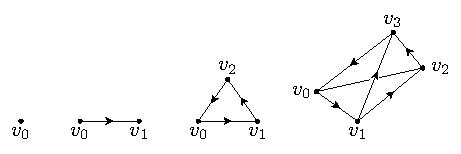
\includegraphics[scale=1.5]{images/fig_1.pdf}\\
                Figura \thefigcount. $n$ simplejos para $n=0,1,2$ y $3$.
                \stepcounter{figcount}
            \end{center}
        \end{minipage}

        De izquierda a derecha se muestran como serían el 0-simplejo, 1-simplejo, 2-simplejo y 3-simplejo metidos en $\mathbb{R}^3$.
    \end{obs}

    \begin{exa}
        El $n$-simplejo que contiene a los vectores canónicos $e_1,...,e_n$ y al cero en $\mathbb{R}^m$ es el conjunto:
        \begin{equation*}
            \Delta^n=\left\{(t_0,...,t_n)\in\mathbb{R}^{ n+1}\Big|\sum_{ i=0}^n t_i\textup{ y }t_i\geq0\textup{ }\forall i=0,...,n \right\}
        \end{equation*}
        es llamado \textbf{$n$-simplejo estándar}. Notemos que $\Delta^n=[0,e_1,...,e_n]$ donde $O$ es el origen de $\mathbb{R}^{ n+1}$.
    \end{exa}

    En homología va a resultar importante mantener el orden de los vértices del simplejo, por lo que cuando digamos \textit{$n$-simplejo}, realmente estaremos diciendo \textit{$n$-simplejo con un ordenamiento de vértices}.

    Una consecuencia de ordenar los vértices de un simplejo $[v_0,...,v_n]$ es que éstos determinan la orientación de los vértices $[v_i,v_j]$ de acuerdo a los subíndices ordenados de forma creciente.

    Especificar este orden de los vértices determina un homomorfismo lineal del $n$-simplejo estándar en cualquier otro $n$-simplejo $[v_0,...,v_n]$ que preserve el orden de los vértices, a saber:
    \begin{equation*}
        (t_0,...,t_n)\mapsto \sum_{ i=0}^n t_iv_i
    \end{equation*}
    los coeficientes $t_i$ son llamados $i$-ésimas \textbf{coordenadas baricéntricas} del punto $\sum_{ i=0}^n t_iv_i$ en el simplejo $[v_0,...,v_n]$.

    \begin{mydef}
        Sea $[v_0,...,v_n]$ un $n$-simplejo y tomemos $j=0,...,n$. Entonces el simplejo $[v_0,...,\hat{v_j},...,v_n]$ es un $(n-1)$-simplejo llamado \textbf{$j$-ésima cara de $[v_0,...,v_n]$}.
    \end{mydef}

    \begin{obs}
        Bajo la definición que hicimos anteriormente, todo subsimplejo de un simplejo estará siempre con los vértices ordenados de forma creciente, de acuerdo al orden que establecimos en el simplejo original. 
    \end{obs}

    \begin{mydef}
        El conjunto formado por la unión de todas las caras de un simplejo $\Delta^n$ es la \textbf{frontera de $\Delta^n$} y se denota por $\partial\Delta^n$. El \textbf{simplejo abierto} $\mathring{\Delta}^n$ es el conjunto $\Delta^n\setminus\partial\Delta^n$.
    \end{mydef}

    \begin{mydef}
        Una \textbf{estructura de $\Delta$-complejo en un espacio $X$} es una colección $\left\{\cf{\sigma_\alpha}{\Delta^{ n_\alpha}}{X} \right\}_{\alpha\in I}$ (con $n_\alpha\in\mathbb{N}\cup\left\{0 \right\}$ para todo $\alpha\in I$) tal que:
        \begin{enumerate}[label = \textit{(\arabic*)}]
            \item 
        \end{enumerate}
    \end{mydef}



\end{document}